\documentclass[a4paper, 10pt]{article}
\usepackage[margin=0.5in]{geometry}

\usepackage{blindtext}
\usepackage{multicol}
\usepackage{booktabs}
\usepackage{amsmath}
\usepackage{mathtools}
\usepackage{float}
\usepackage{graphicx}
\usepackage{enumitem}
\usepackage{hyperref}
\usepackage{comment}

\graphicspath{{./outputs}}


\setlength{\columnsep}{1cm}
\title{ENPM 673: Perception for Autonomous Robots - MidTerm Exam}
\author{Aswath Muthuselvam \\ aswath@umd.edu \\ 118286204}
\date{16th March 2022}

\begin{document}
	\maketitle
	\newlist{contract}{enumerate}{10}
	\setlist[contract]{label*=\arabic*.}
	\setlistdepth{10} 
	
	\begin{multicols}{2}
		
		\section{Question 1: Counting coins}
		\subsection{Separate the coins}
		
		The coins are separated by lines of varying thicknesses, hence it can be removed by using a structuring element filled with zeros. I separated the coins using erosion. I used a kernel of size 20x20 with one iteration of erosion. 

		\subsection{Counting the coins}
		
		Now that the coins are separated, I used opencv's findcontours() function to find all the 24 convex shapes. The findcontours() function takes all non zero pixels as 1 and zero pixels as zero, hence, I converted the eroded image to grayscale and thresholded it to remove any darker pixels. the The number of detected contours detected is also the number of coins present in the original image. The number of coins detected will be printed by the question1.py script that is included with this report. Figure \ref{fig:op1} shows the complete process of erosion and contour detection.
				
		\begin{figure}[H]
			\centering
			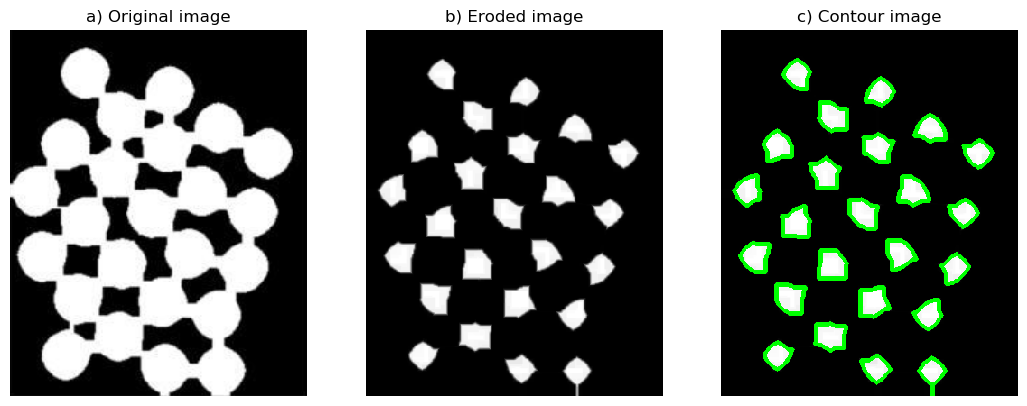
\includegraphics[width=\columnwidth]{/output1.png}
			\caption{Counting coins in the image}
			\label{fig:op1}
		\end{figure}

		\begin{figure}[H]
			\centering
			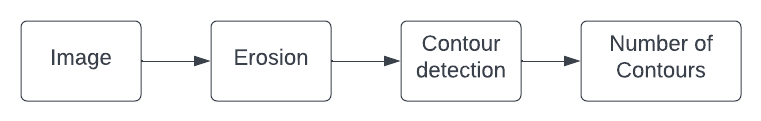
\includegraphics[width=\columnwidth]{/block1.png}
			\caption{Block diagram of coin counting pipeline}
			\label{fig:block1}
		\end{figure}
	
		\begin{comment}
		
		\begin{figure*}
		\centering
		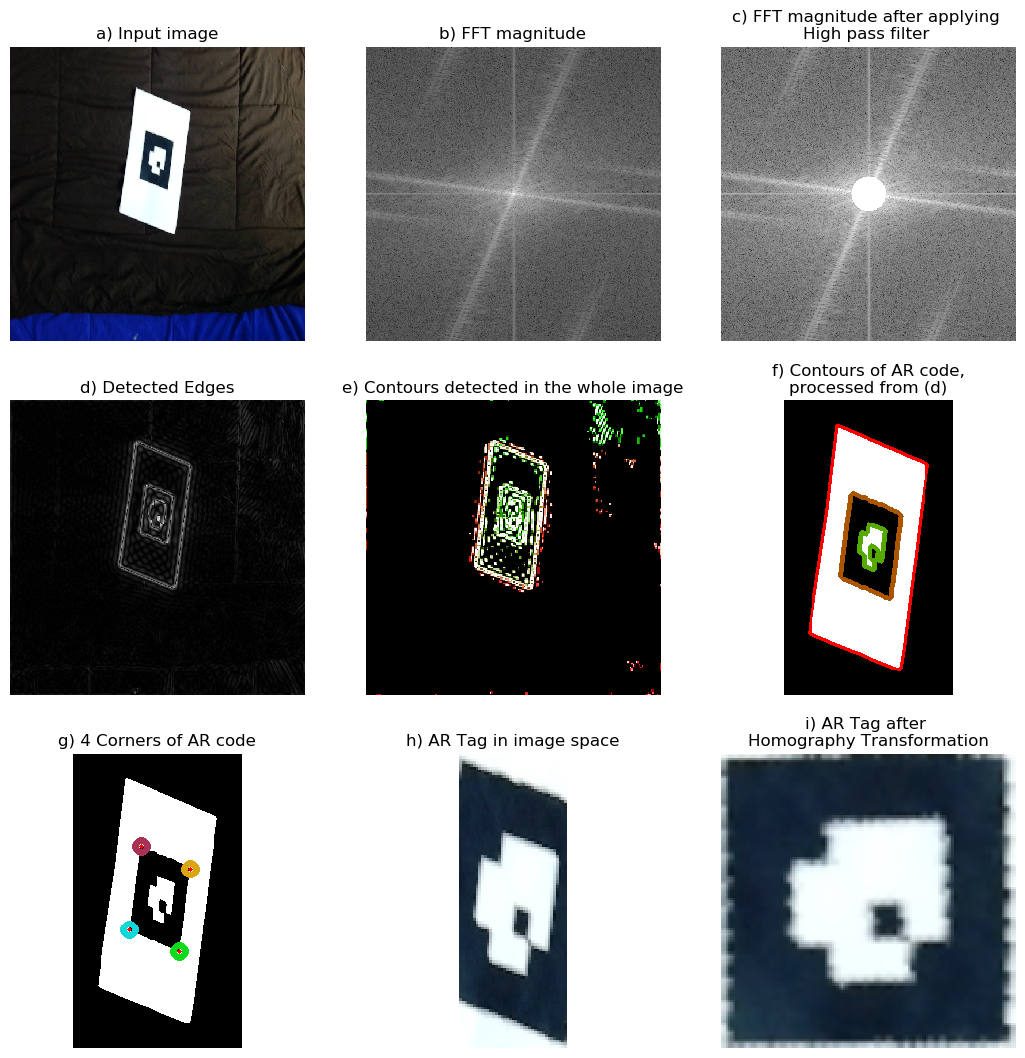
\includegraphics[width=0.75\textwidth]{/Q1/ARDetectionUsingFFt.png}
		\caption{Projecting the Testudo image on the ARTag}
		\label{fig:ARTa1g}
		\end{figure*}
		
		\end{comment}
		
		
		\section{Question 2: Image Stitching}
		There are two images given, one of the images is taken by translating the camera to the left side. We are going to stitch both of them together. 
		
		First, I converted the images to grayscale. Then, I used Feature detection to find significant Features in the image. Using the keypoints and descriptors obtained, I matched the keypoints using a Brute force matcher with L1 norm, this gives the relation between the points in the Image A and Image B. I used opencv findHomography() to find the Homography between the source and destination points. Then, with the Homograhy matrix, I warped the images using warpPerspective() function. Figure \ref{fig:op2} shows the complete process of Feature detection, Keypoint Matching, finding Homography and Warping the final image.
		
		The homography transformation matrix is given by:
		\[
		\begin{bmatrix}
		x^{'} \\
		y^{'} \\
		w
		\end{bmatrix} =
		H\begin{bmatrix}
		x \\
		y \\
		1
		\end{bmatrix} = 
		\begin{bmatrix}
		h_{11} & h_{12} & h_{13}\\
		h_{21} & h_{22} & h_{23}\\
		h_{31} & h_{32} & h_{33}
		\end{bmatrix}
		\begin{bmatrix}
		x \\
		y \\
		1
		\end{bmatrix}
		\]
		
		\begin{figure}[H]
			\centering
			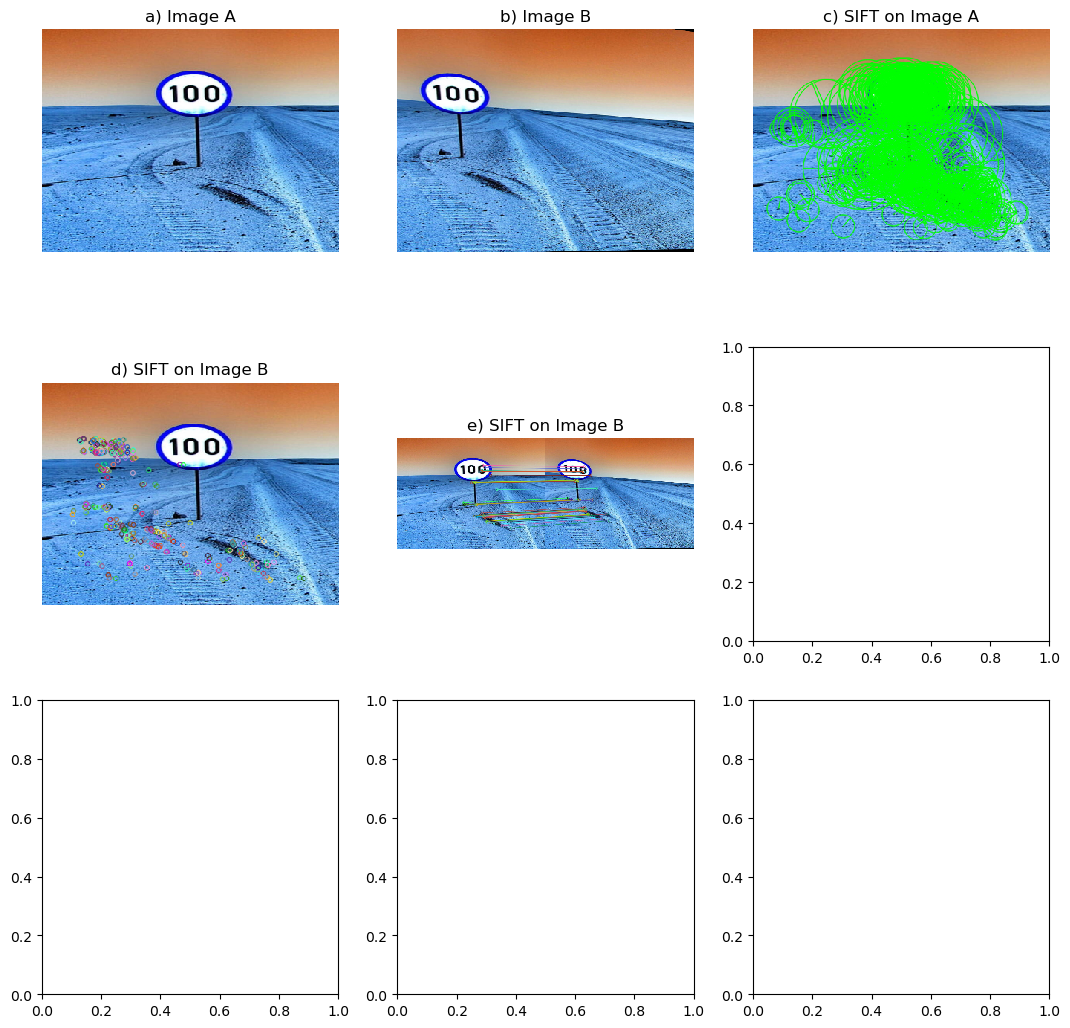
\includegraphics[width=\columnwidth]{/output2.png}
			\caption{Stitching two images}
			\label{fig:op2}
		\end{figure}
		
		\begin{figure}[H]
			\centering
			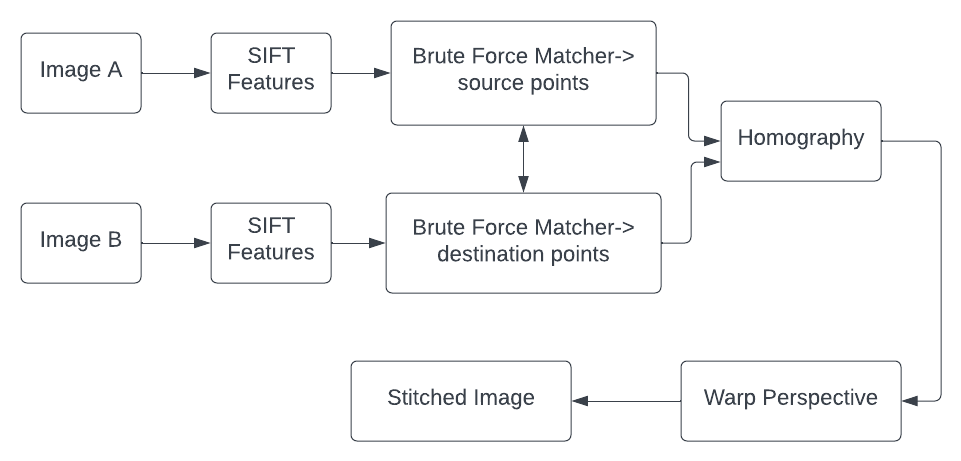
\includegraphics[width=\columnwidth]{/block2.png}
			\caption{Block diagram of Image stitching pipeline}
			\label{fig:block2}
		\end{figure}
		
		
		\section{Question 3: Camera parameters}
		
		\textbf{1. What is the minimum number matching points to solve this mathematically?}
		
		\textbf{Answer:}
			6 points are required to solve this.
			
		\textbf{2. What is the pipeline or the block diagram that needs to be done in order to calibrate this camera given the image above.}
		
		\textbf{Answer:}
		The block diagram is shown below in Figure \ref{fig:block3}.
		
		\begin{figure}[H]
			\centering
			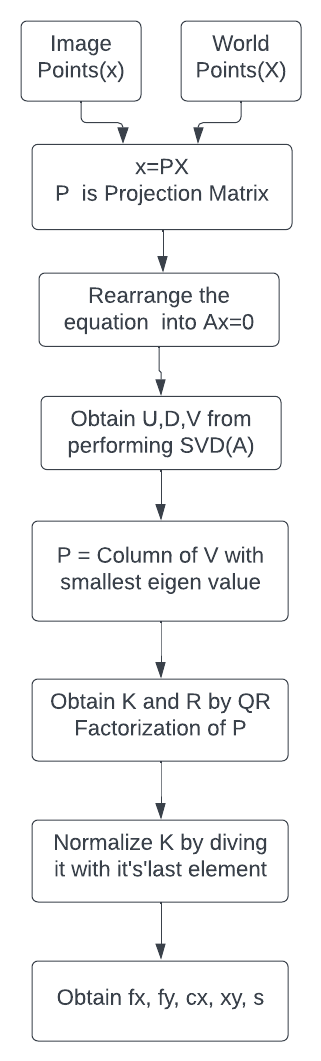
\includegraphics[width=0.5\columnwidth]{/block3.png}
			\caption{Block diagram of Finding Camera matrix - K}
			\label{fig:block3}
		\end{figure}
		
		
		\textbf{3. First write down the mathematical formation for your answer including steps that needs to be done to find the intrinsic matrix K}
		
		\textbf{Answer:}
		$x$ is the coordinates of points in the image.
		$X$ is the coordinates of points in the world frame.
		$P$ is the Projection matrix.
		\[x = PX\]
		
		$P$ can be decomposed as
		\[
		w\begin{bmatrix}
		x/w \\
		y/w \\
		1
		\end{bmatrix} =
		\begin{bmatrix}
		x \\
		y \\
		w
		\end{bmatrix} = 
		\begin{bmatrix}
		p_{1} & p_{2} & p_{3} & p_{4}\\
		p_{5} & p_{6} & p_{7} & p_{8}\\
		p_{9} & p_{10} & p_{11} & p_{12}
		\end{bmatrix}
		\begin{bmatrix}
		X \\
		Y \\
		Z \\
		1
		\end{bmatrix}
		\]
		
		
		
		By the pinhole camera model, $P$ reduces to:
		
		\[
		\mathbf{x}{\mathbf{i}} \times \mathbf{P} \mathbf{X}{\mathbf{i}}=\left[\begin{array}{l}
		v_{\mathbf{i}}^{\mathrm{i}} \mathbf{p}{3}^{\mathrm{T}} \mathbf{X}{\mathbf{i}}-w_{\mathbf{i}}^{\prime} \mathbf{p}{2}^{\mathrm{T}} \mathbf{X}{\mathbf{i}} \\
		w_{\mathrm{i}}^{\prime} \mathbf{p}{1}^{\mathrm{T}} \mathbf{X}{\mathbf{i}}-u_{\mathbf{i}}^{\prime} \mathbf{p}{3}^{\mathrm{T}} \mathbf{X}{\mathbf{i}} \\
		u_{\mathrm{i}}^{\prime} \mathbf{p}{2}^{\mathrm{T}} \mathbf{X}{\mathbf{i}}-v_{\mathbf{i}}^{\prime} \mathbf{p}{1}^{\mathrm{T}} \mathbf{X}{\mathbf{i}}
		\end{array}\right]
		\]
		
		
		The above equation can be rewritten as:
		
		\[
		\left[\begin{array}{ccc}
		\mathbf{0}{4}^{\mathrm{T}} & -w{\mathrm{i}}^{\prime} \mathbf{X}{\mathrm{i}}^{\mathrm{T}} & v{\mathrm{i}}^{\prime} \mathbf{X}_{\mathrm{i}}^{\mathrm{T}} \\
		w_{\mathbf{i}}^{\prime} \mathbf{X}{\mathrm{i}}^{\mathrm{T}} & 0{4}^{\mathrm{T}} & -u_{\mathrm{i}}^{\prime} \mathbf{X}_{\mathrm{i}}^{\mathrm{T}} \\
		-v_{\mathbf{i}}^{\prime} \mathbf{X}{\mathrm{i}}^{\mathrm{T}} & u{\mathrm{i}}^{\prime} \mathbf{X}{\mathbf{i}}^{\mathrm{T}} & \mathbf{0}{\mathbf{T}}^{\mathrm{T}}
		\end{array}\right]\left[\begin{array}{l}
		\mathbf{p}_{1} \\
		\mathbf{p}_{2} \\
		\mathbf{p}_{3}
		\end{array}\right]=0		
		\]
		
		This can be represented in the form:
		$Ax=0$
		
		
		
		We then perform SVD of A. The last column of V is the P matrix. V can be reshaped into 3x4 matrix. In a homogeneous equation such as $Ax=0$, any vector $x$ in the null space of $A$ is a solution. Hence any column of $V$ whose corresponding singular value is zero is a solution. In our case, since the data is from real world with noise added to it, we can take the column with the least Eigen value. 
		
		
		
		The K matrix is of the form:
		\[
		K = \begin{bmatrix}
		f & 0 & p_{x} & 0 \\
		f & f & p_{y} & 0 \\
		0 & 0 & 1 & 0
		\end{bmatrix}
		\]
		
		The matrix obtained is:
		\[
		K =
		\begin{bmatrix}
		34.1030  &  5.8943 & 755.1036 \\
		0  & 34.4705  &  8.6312 \\
		0  &       0  &  1.0000
		\end{bmatrix}
		\]
	
	\section{Question 4: K-Means segmentation}
	
	Since the classification is based on the color, the feature space for the K-means is the color space, i.e. Red, Green and Blue components. This means, that, the distance between the feature points is calculated between the components of the 3 color spaces. I did think about converting the image to LAB and segmenting in that feature space. However, RGB works fine as well. Before clustering, I resized the image to 100x100 pixels before processing it. Figure \ref{fig:colorspace} shows the colors present in the traffic signal image and Figure \ref{fig:kmeans} shows the plot of the 4 Means that the algorithm converged into.
	
	\begin{figure}[H]
	\centering
	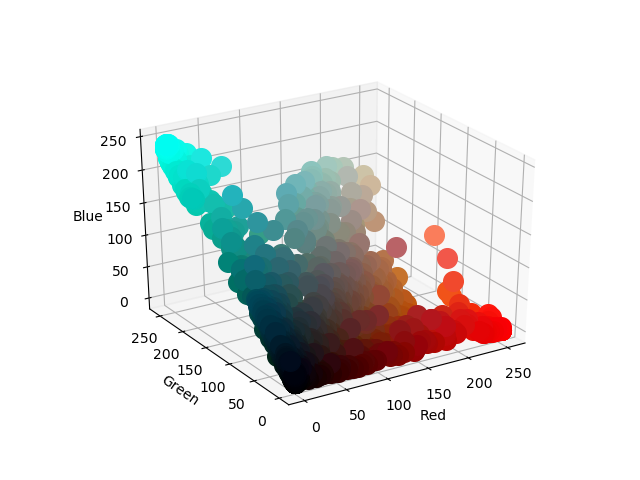
\includegraphics[width=0.75\columnwidth]{/colorspaceKNNbig.png}
	\caption{Color space of the input image}
	\label{fig:colorspace}
	\end{figure}
	
	\begin{figure}[H]
	\centering
	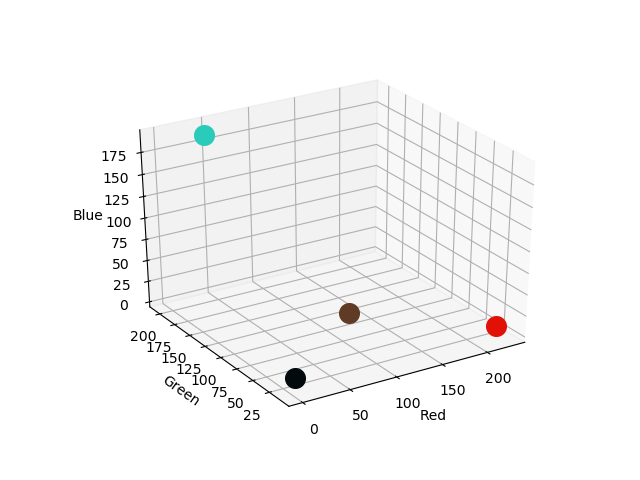
\includegraphics[width=0.75\columnwidth]{/KMeans.png}
	\caption{K-Means, K=4}
	\label{fig:kmeans}
	\end{figure}		
	
	The algorithm of K-Means that I implemented is described as follows. We are given a set of feature points $X$, which we want to cluster it into $K$ classes. We start by creating a Dictionary D with $K$ keys, each key will contain a list of values which will be obtained from the feature points based on the method which will be described next. We also have a list of Means $M$ of size $K$ containing the means of each cluster. Initially, the values of each means $m_{i}$ are assigned randomly. Next, we loop through each feature point and computes its distance form each of the means, the nearest distance $d$ is assigned to the respective class in the dictionary. The distance between a given feature point and mean can be calculated with Euclidean or Manhattan distance. The mean of each classes in the dictionary is computed and updated to the respective mean $m_{i}$. The above described procedure can be iterated for any number of time steps $T$ to obtain a closer fit to the data, or it can be stopped when the means $m_{i}$ are not changing with every iteration.
	
	The output is shown of 4 class - classification is showed in Figure \ref{fig:op4}. The 4 classes are black, red, blue and brown color, image(b) shows the classes in a discretized manner.
	
	\begin{figure}[H]
		\centering
		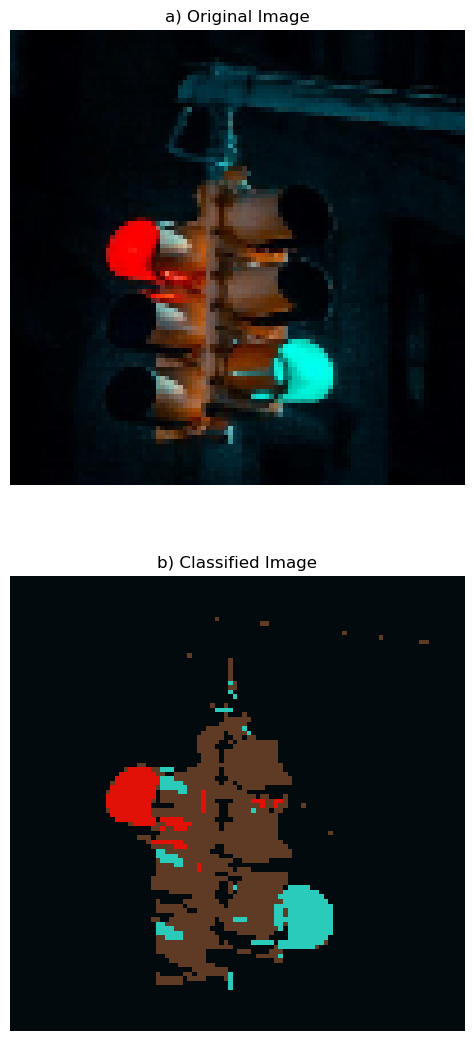
\includegraphics[width=\columnwidth]{/output4.png}
		\caption{K-Means segmentation, K=4}
		\label{fig:op4}
	\end{figure}
		
	\end{multicols}
	
\end{document}
